\documentclass[twoside]{book}

% Packages required by doxygen
\usepackage{fixltx2e}
\usepackage{calc}
\usepackage{doxygen}
\usepackage[export]{adjustbox} % also loads graphicx
\usepackage{graphicx}
\usepackage[utf8]{inputenc}
\usepackage{makeidx}
\usepackage{multicol}
\usepackage{multirow}
\PassOptionsToPackage{warn}{textcomp}
\usepackage{textcomp}
\usepackage[nointegrals]{wasysym}
\usepackage[table]{xcolor}

% Font selection
\usepackage[T1]{fontenc}
\usepackage[scaled=.90]{helvet}
\usepackage{courier}
\usepackage{amssymb}
\usepackage{sectsty}
\renewcommand{\familydefault}{\sfdefault}
\allsectionsfont{%
  \fontseries{bc}\selectfont%
  \color{darkgray}%
}
\renewcommand{\DoxyLabelFont}{%
  \fontseries{bc}\selectfont%
  \color{darkgray}%
}
\newcommand{\+}{\discretionary{\mbox{\scriptsize$\hookleftarrow$}}{}{}}

% Page & text layout
\usepackage{geometry}
\geometry{%
  a4paper,%
  top=2.5cm,%
  bottom=2.5cm,%
  left=2.5cm,%
  right=2.5cm%
}
\tolerance=750
\hfuzz=15pt
\hbadness=750
\setlength{\emergencystretch}{15pt}
\setlength{\parindent}{0cm}
\setlength{\parskip}{3ex plus 2ex minus 2ex}
\makeatletter
\renewcommand{\paragraph}{%
  \@startsection{paragraph}{4}{0ex}{-1.0ex}{1.0ex}{%
    \normalfont\normalsize\bfseries\SS@parafont%
  }%
}
\renewcommand{\subparagraph}{%
  \@startsection{subparagraph}{5}{0ex}{-1.0ex}{1.0ex}{%
    \normalfont\normalsize\bfseries\SS@subparafont%
  }%
}
\makeatother

% Headers & footers
\usepackage{fancyhdr}
\pagestyle{fancyplain}
\fancyhead[LE]{\fancyplain{}{\bfseries\thepage}}
\fancyhead[CE]{\fancyplain{}{}}
\fancyhead[RE]{\fancyplain{}{\bfseries\leftmark}}
\fancyhead[LO]{\fancyplain{}{\bfseries\rightmark}}
\fancyhead[CO]{\fancyplain{}{}}
\fancyhead[RO]{\fancyplain{}{\bfseries\thepage}}
\fancyfoot[LE]{\fancyplain{}{}}
\fancyfoot[CE]{\fancyplain{}{}}
\fancyfoot[RE]{\fancyplain{}{\bfseries\scriptsize Generated by Doxygen }}
\fancyfoot[LO]{\fancyplain{}{\bfseries\scriptsize Generated by Doxygen }}
\fancyfoot[CO]{\fancyplain{}{}}
\fancyfoot[RO]{\fancyplain{}{}}
\renewcommand{\footrulewidth}{0.4pt}
\renewcommand{\chaptermark}[1]{%
  \markboth{#1}{}%
}
\renewcommand{\sectionmark}[1]{%
  \markright{\thesection\ #1}%
}

% Indices & bibliography
\usepackage{natbib}
\usepackage[titles]{tocloft}
\setcounter{tocdepth}{3}
\setcounter{secnumdepth}{5}
\makeindex

% Custom commands
\newcommand{\clearemptydoublepage}{%
  \newpage{\pagestyle{empty}\cleardoublepage}%
}

\usepackage{caption}
\captionsetup{labelsep=space,justification=centering,font={bf},singlelinecheck=off,skip=4pt,position=top}

%===== C O N T E N T S =====

\begin{document}

% Titlepage & ToC
\pagenumbering{roman}
\begin{titlepage}
\vspace*{7cm}
\begin{center}%
{\Large Sudoku Project }\\
\vspace*{1cm}
{\large Generated by Doxygen 1.8.11}\\
\end{center}
\end{titlepage}
\clearemptydoublepage
\tableofcontents
\clearemptydoublepage
\pagenumbering{arabic}

%--- Begin generated contents ---
\chapter{File Index}
\section{File List}
Here is a list of all files with brief descriptions\+:\begin{DoxyCompactList}
\item\contentsline{section}{{\bf Display.\+c} }{\pageref{_display_8c}}{}
\item\contentsline{section}{{\bf essential\+Functions.\+c} }{\pageref{essential_functions_8c}}{}
\item\contentsline{section}{{\bf Generate\+Sudoku\+Puzzle.\+c} }{\pageref{_generate_sudoku_puzzle_8c}}{}
\item\contentsline{section}{{\bf main.\+c} }{\pageref{main_8c}}{}
\item\contentsline{section}{{\bf sudoku.\+h} }{\pageref{sudoku_8h}}{}
\item\contentsline{section}{{\bf Sudoku\+Solver.\+c} }{\pageref{_sudoku_solver_8c}}{}
\end{DoxyCompactList}

\chapter{File Documentation}
\section{Display.\+c File Reference}
\label{_display_8c}\index{Display.\+c@{Display.\+c}}
{\ttfamily \#include \char`\"{}sudoku.\+h\char`\"{}}\\*
Include dependency graph for Display.\+c\+:
\nopagebreak
\begin{figure}[H]
\begin{center}
\leavevmode
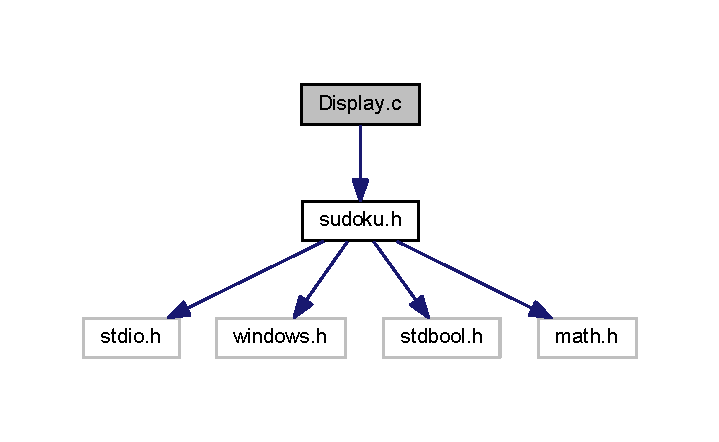
\includegraphics[width=345pt]{_display_8c__incl}
\end{center}
\end{figure}
\subsection*{Functions}
\begin{DoxyCompactItemize}
\item 
void {\bf Intro} ()
\begin{DoxyCompactList}\small\item\em Generate intro interface. \end{DoxyCompactList}\item 
void {\bf Chose\+Options} ()
\begin{DoxyCompactList}\small\item\em Generate chose options interface for switch . \end{DoxyCompactList}\item 
void {\bf Back} (int puzzle, int copy, int {\bf Size\+Of\+Puzzle})
\begin{DoxyCompactList}\small\item\em Call back-\/up of last puzzle. \end{DoxyCompactList}\item 
void {\bf Insert\+Number\+In\+Pozition\+Choice} (int puzzle, int copy, int {\bf Size\+Of\+Puzzle})
\begin{DoxyCompactList}\small\item\em Insert number in pozition at your choice ! \end{DoxyCompactList}\item 
void {\bf Generate\+Random\+Puzzle} (int puzzle, int copy, F\+I\+LE $\ast$name\+Of\+File, int {\bf Size\+Of\+Puzzle})
\begin{DoxyCompactList}\small\item\em Generate puzzle. \end{DoxyCompactList}\item 
void {\bf Solve\+Puzzle} (int puzzle, F\+I\+LE $\ast$file\+To\+Print, int {\bf Size\+Of\+Puzzle})
\begin{DoxyCompactList}\small\item\em A function which will call solving parts to solve the puzzle ! \end{DoxyCompactList}\item 
void {\bf Ask\+Size} (int {\bf Size\+Of\+Puzzle}, int puzzle)
\begin{DoxyCompactList}\small\item\em Ask for size of puzzle . \end{DoxyCompactList}\end{DoxyCompactItemize}


\subsection{Function Documentation}
\index{Display.\+c@{Display.\+c}!Ask\+Size@{Ask\+Size}}
\index{Ask\+Size@{Ask\+Size}!Display.\+c@{Display.\+c}}
\subsubsection[{Ask\+Size(int Size\+Of\+Puzzle, int puzzle)}]{\setlength{\rightskip}{0pt plus 5cm}void Ask\+Size (
\begin{DoxyParamCaption}
\item[{int}]{Size\+Of\+Puzzle, }
\item[{int}]{puzzle}
\end{DoxyParamCaption}
)}\label{_display_8c_a24f742529f237af6fdbcf8ed04f07be9}


Ask for size of puzzle . 


\begin{DoxyParams}{Parameters}
{\em puzzle} & The respective puzzle \\
\hline
{\em Size\+Of\+Puzzle} & Puzzle size. \\
\hline
\end{DoxyParams}


Here is the call graph for this function\+:
\nopagebreak
\begin{figure}[H]
\begin{center}
\leavevmode
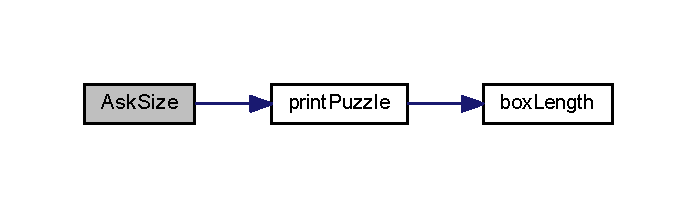
\includegraphics[width=334pt]{_display_8c_a24f742529f237af6fdbcf8ed04f07be9_cgraph}
\end{center}
\end{figure}




Here is the caller graph for this function\+:
\nopagebreak
\begin{figure}[H]
\begin{center}
\leavevmode
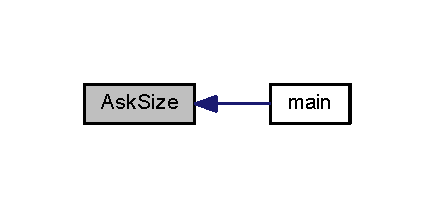
\includegraphics[width=208pt]{_display_8c_a24f742529f237af6fdbcf8ed04f07be9_icgraph}
\end{center}
\end{figure}


\index{Display.\+c@{Display.\+c}!Back@{Back}}
\index{Back@{Back}!Display.\+c@{Display.\+c}}
\subsubsection[{Back(int puzzle, int copy, int Size\+Of\+Puzzle)}]{\setlength{\rightskip}{0pt plus 5cm}void Back (
\begin{DoxyParamCaption}
\item[{int}]{puzzle, }
\item[{int}]{copy, }
\item[{int}]{Size\+Of\+Puzzle}
\end{DoxyParamCaption}
)}\label{_display_8c_a715f37ae3e08e5f6d3e95eb5f4d8adc3}


Call back-\/up of last puzzle. 



Here is the call graph for this function\+:
\nopagebreak
\begin{figure}[H]
\begin{center}
\leavevmode
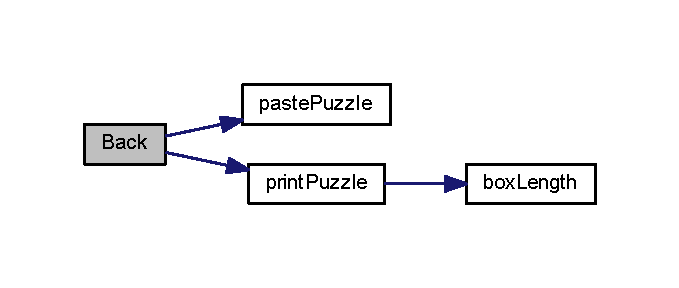
\includegraphics[width=326pt]{_display_8c_a715f37ae3e08e5f6d3e95eb5f4d8adc3_cgraph}
\end{center}
\end{figure}




Here is the caller graph for this function\+:
\nopagebreak
\begin{figure}[H]
\begin{center}
\leavevmode
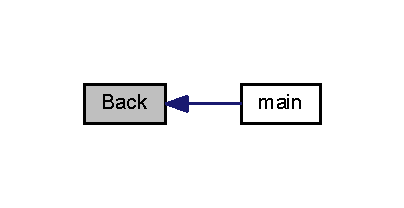
\includegraphics[width=194pt]{_display_8c_a715f37ae3e08e5f6d3e95eb5f4d8adc3_icgraph}
\end{center}
\end{figure}


\index{Display.\+c@{Display.\+c}!Chose\+Options@{Chose\+Options}}
\index{Chose\+Options@{Chose\+Options}!Display.\+c@{Display.\+c}}
\subsubsection[{Chose\+Options()}]{\setlength{\rightskip}{0pt plus 5cm}void Chose\+Options (
\begin{DoxyParamCaption}
{}
\end{DoxyParamCaption}
)}\label{_display_8c_ab972c0e63449ab0cbfed7cdcc3d3f534}


Generate chose options interface for switch . 



Here is the caller graph for this function\+:
\nopagebreak
\begin{figure}[H]
\begin{center}
\leavevmode
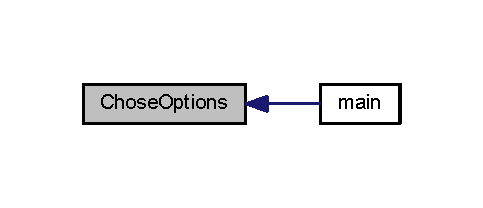
\includegraphics[width=232pt]{_display_8c_ab972c0e63449ab0cbfed7cdcc3d3f534_icgraph}
\end{center}
\end{figure}


\index{Display.\+c@{Display.\+c}!Generate\+Random\+Puzzle@{Generate\+Random\+Puzzle}}
\index{Generate\+Random\+Puzzle@{Generate\+Random\+Puzzle}!Display.\+c@{Display.\+c}}
\subsubsection[{Generate\+Random\+Puzzle(int puzzle, int copy, F\+I\+L\+E $\ast$name\+Of\+File, int Size\+Of\+Puzzle)}]{\setlength{\rightskip}{0pt plus 5cm}void Generate\+Random\+Puzzle (
\begin{DoxyParamCaption}
\item[{int}]{puzzle, }
\item[{int}]{copy, }
\item[{F\+I\+LE $\ast$}]{name\+Of\+File, }
\item[{int}]{Size\+Of\+Puzzle}
\end{DoxyParamCaption}
)}\label{_display_8c_ae19873683ff86a7e6f531517e9eb079b}


Generate puzzle. 



Here is the call graph for this function\+:
\nopagebreak
\begin{figure}[H]
\begin{center}
\leavevmode
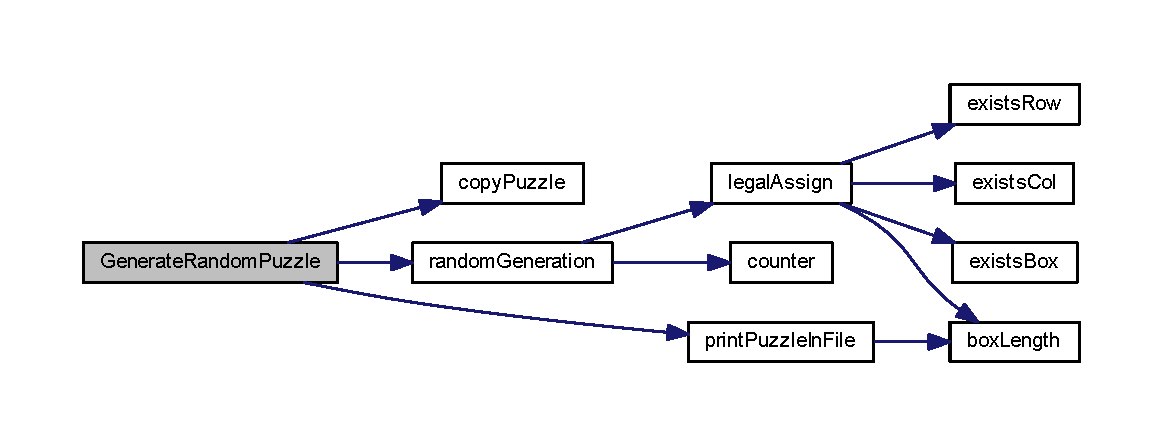
\includegraphics[width=350pt]{_display_8c_ae19873683ff86a7e6f531517e9eb079b_cgraph}
\end{center}
\end{figure}




Here is the caller graph for this function\+:
\nopagebreak
\begin{figure}[H]
\begin{center}
\leavevmode
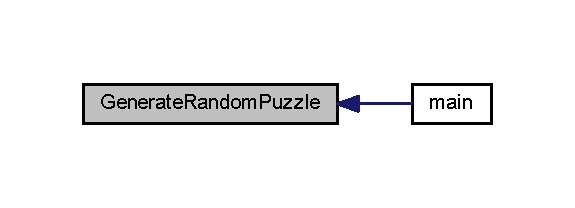
\includegraphics[width=276pt]{_display_8c_ae19873683ff86a7e6f531517e9eb079b_icgraph}
\end{center}
\end{figure}


\index{Display.\+c@{Display.\+c}!Insert\+Number\+In\+Pozition\+Choice@{Insert\+Number\+In\+Pozition\+Choice}}
\index{Insert\+Number\+In\+Pozition\+Choice@{Insert\+Number\+In\+Pozition\+Choice}!Display.\+c@{Display.\+c}}
\subsubsection[{Insert\+Number\+In\+Pozition\+Choice(int puzzle, int copy, int Size\+Of\+Puzzle)}]{\setlength{\rightskip}{0pt plus 5cm}void Insert\+Number\+In\+Pozition\+Choice (
\begin{DoxyParamCaption}
\item[{int}]{puzzle, }
\item[{int}]{copy, }
\item[{int}]{Size\+Of\+Puzzle}
\end{DoxyParamCaption}
)}\label{_display_8c_a8ba4a5060a15be37bd198bc8becc32e0}


Insert number in pozition at your choice ! 



Here is the call graph for this function\+:
\nopagebreak
\begin{figure}[H]
\begin{center}
\leavevmode
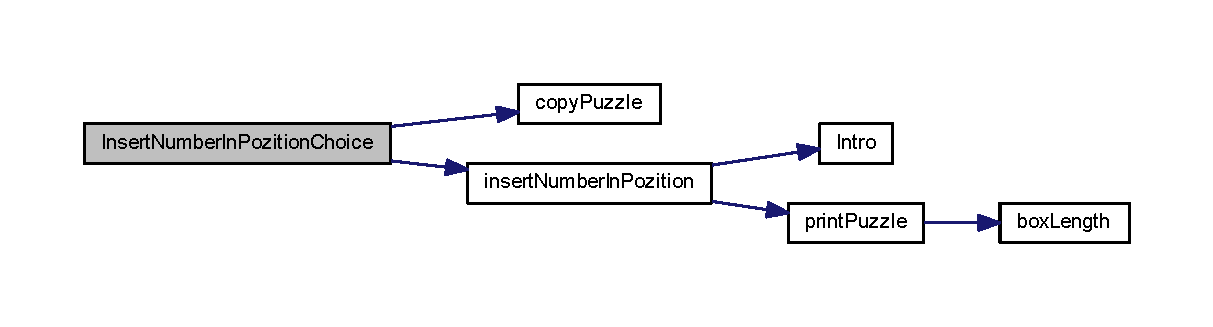
\includegraphics[width=350pt]{_display_8c_a8ba4a5060a15be37bd198bc8becc32e0_cgraph}
\end{center}
\end{figure}




Here is the caller graph for this function\+:
\nopagebreak
\begin{figure}[H]
\begin{center}
\leavevmode
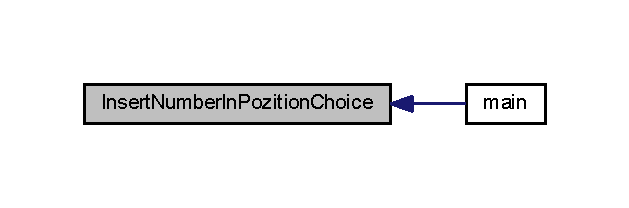
\includegraphics[width=302pt]{_display_8c_a8ba4a5060a15be37bd198bc8becc32e0_icgraph}
\end{center}
\end{figure}


\index{Display.\+c@{Display.\+c}!Intro@{Intro}}
\index{Intro@{Intro}!Display.\+c@{Display.\+c}}
\subsubsection[{Intro()}]{\setlength{\rightskip}{0pt plus 5cm}void Intro (
\begin{DoxyParamCaption}
{}
\end{DoxyParamCaption}
)}\label{_display_8c_a8cc9a674e9251c1094cb42a4b272e94d}


Generate intro interface. 



Here is the caller graph for this function\+:
\nopagebreak
\begin{figure}[H]
\begin{center}
\leavevmode
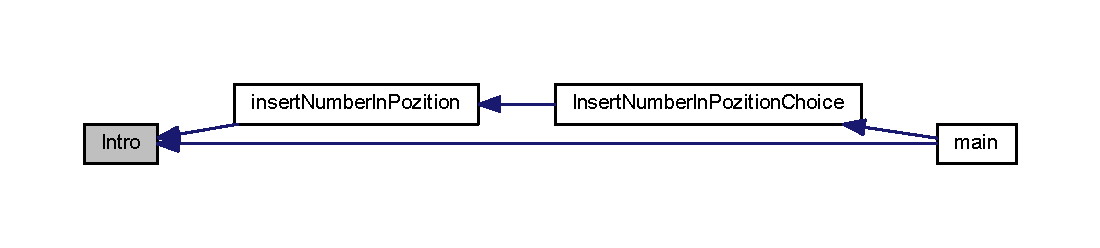
\includegraphics[width=350pt]{_display_8c_a8cc9a674e9251c1094cb42a4b272e94d_icgraph}
\end{center}
\end{figure}


\index{Display.\+c@{Display.\+c}!Solve\+Puzzle@{Solve\+Puzzle}}
\index{Solve\+Puzzle@{Solve\+Puzzle}!Display.\+c@{Display.\+c}}
\subsubsection[{Solve\+Puzzle(int puzzle, F\+I\+L\+E $\ast$file\+To\+Print, int Size\+Of\+Puzzle)}]{\setlength{\rightskip}{0pt plus 5cm}void Solve\+Puzzle (
\begin{DoxyParamCaption}
\item[{int}]{puzzle, }
\item[{F\+I\+LE $\ast$}]{file\+To\+Print, }
\item[{int}]{Size\+Of\+Puzzle}
\end{DoxyParamCaption}
)}\label{_display_8c_a6d3e94a6ec4802bab363ab8a1fe873fa}


A function which will call solving parts to solve the puzzle ! 

The solution is printed on console display. /$\ast$$\ast$ Generate print interface.

\textbackslash{} print\+Puzzle(puzzle, Size\+Of\+Puzzle);

\textbackslash{} The solution is printed on Solutions file ! 

Here is the call graph for this function\+:
\nopagebreak
\begin{figure}[H]
\begin{center}
\leavevmode
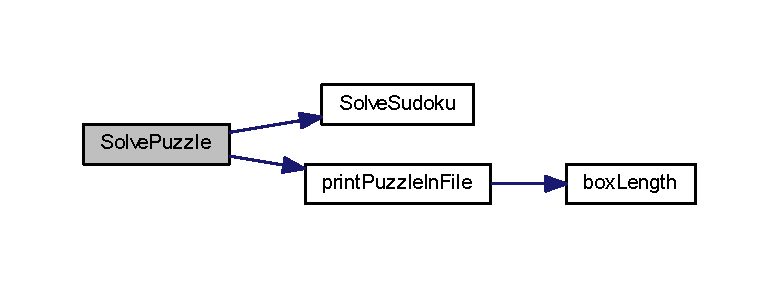
\includegraphics[width=350pt]{_display_8c_a6d3e94a6ec4802bab363ab8a1fe873fa_cgraph}
\end{center}
\end{figure}




Here is the caller graph for this function\+:
\nopagebreak
\begin{figure}[H]
\begin{center}
\leavevmode
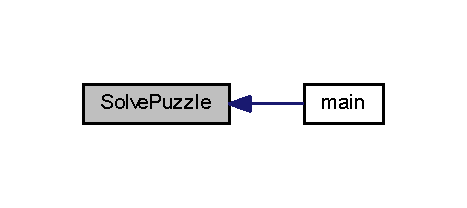
\includegraphics[width=224pt]{_display_8c_a6d3e94a6ec4802bab363ab8a1fe873fa_icgraph}
\end{center}
\end{figure}



\section{essential\+Functions.\+c File Reference}
\label{essential_functions_8c}\index{essential\+Functions.\+c@{essential\+Functions.\+c}}
{\ttfamily \#include \char`\"{}sudoku.\+h\char`\"{}}\\*
Include dependency graph for essential\+Functions.\+c\+:
\nopagebreak
\begin{figure}[H]
\begin{center}
\leavevmode
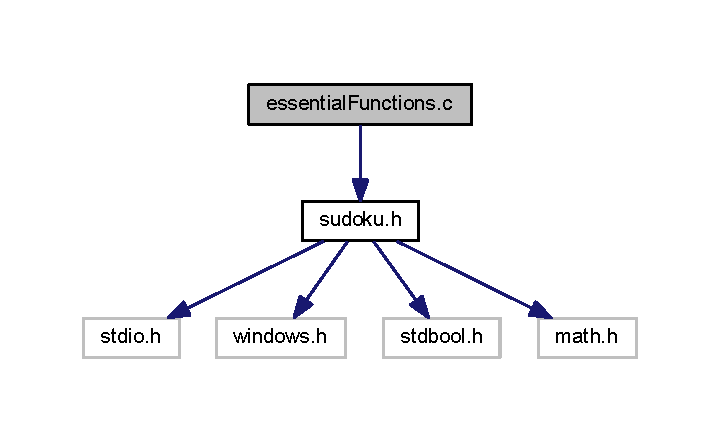
\includegraphics[width=345pt]{essential_functions_8c__incl}
\end{center}
\end{figure}
\subsection*{Functions}
\begin{DoxyCompactItemize}
\item 
int {\bf box\+Length} (int {\bf Size\+Of\+Puzzle})
\begin{DoxyCompactList}\small\item\em A function which will determine box size. \end{DoxyCompactList}\item 
void {\bf copy\+Puzzle} (int puzzle[{\bf Size\+Of\+Puzzle}][{\bf Size\+Of\+Puzzle}], int copy[{\bf Size\+Of\+Puzzle}][{\bf Size\+Of\+Puzzle}])
\begin{DoxyCompactList}\small\item\em A function to Back\+Up the puzzle. \end{DoxyCompactList}\item 
void {\bf paste\+Puzzle} (int puzzle[{\bf Size\+Of\+Puzzle}][{\bf Size\+Of\+Puzzle}], int copy[{\bf Size\+Of\+Puzzle}][{\bf Size\+Of\+Puzzle}])
\begin{DoxyCompactList}\small\item\em An another function to Back\+Up the puzzle. \end{DoxyCompactList}\item 
void {\bf print\+Puzzle} (int puzzle[{\bf Size\+Of\+Puzzle}][{\bf Size\+Of\+Puzzle}], int {\bf Size\+Of\+Puzzle})
\begin{DoxyCompactList}\small\item\em Function which will print puzzle. \end{DoxyCompactList}\item 
void {\bf print\+Puzzle\+In\+File} (F\+I\+LE $\ast$filename, int puzzle[{\bf Size\+Of\+Puzzle}][{\bf Size\+Of\+Puzzle}], int {\bf Size\+Of\+Puzzle})
\begin{DoxyCompactList}\small\item\em Function which will print puzzle in a file. \end{DoxyCompactList}\item 
void {\bf insert\+Number\+In\+Pozition} (int puzzle[{\bf Size\+Of\+Puzzle}][{\bf Size\+Of\+Puzzle}], int {\bf Size\+Of\+Puzzle})
\begin{DoxyCompactList}\small\item\em Function which will insert number in specificated position. \end{DoxyCompactList}\item 
int {\bf Ask} ()
\begin{DoxyCompactList}\small\item\em Ask function as well as it\textquotesingle{}s called just ask user which will be the size of puzzle. \end{DoxyCompactList}\item 
int {\bf counter} (int puzzle[{\bf Size\+Of\+Puzzle}][{\bf Size\+Of\+Puzzle}])
\begin{DoxyCompactList}\small\item\em Counter function will return how many numbers shoud be finded in our sudoku puzzle. \end{DoxyCompactList}\item 
$\ast$param file Data file $\ast$bool {\bf Open\+Files} (F\+I\+LE $\ast$file)
\begin{DoxyCompactList}\small\item\em A function which will check if file is open. \end{DoxyCompactList}\end{DoxyCompactItemize}


\subsection{Function Documentation}
\index{essential\+Functions.\+c@{essential\+Functions.\+c}!Ask@{Ask}}
\index{Ask@{Ask}!essential\+Functions.\+c@{essential\+Functions.\+c}}
\subsubsection[{Ask()}]{\setlength{\rightskip}{0pt plus 5cm}int Ask (
\begin{DoxyParamCaption}
{}
\end{DoxyParamCaption}
)}\label{essential_functions_8c_a77b57b60f97f45e6e20286d7aa4b01ed}


Ask function as well as it\textquotesingle{}s called just ask user which will be the size of puzzle. 



Here is the caller graph for this function\+:
\nopagebreak
\begin{figure}[H]
\begin{center}
\leavevmode
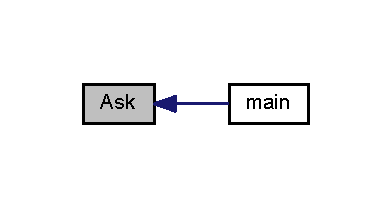
\includegraphics[width=188pt]{essential_functions_8c_a77b57b60f97f45e6e20286d7aa4b01ed_icgraph}
\end{center}
\end{figure}


\index{essential\+Functions.\+c@{essential\+Functions.\+c}!box\+Length@{box\+Length}}
\index{box\+Length@{box\+Length}!essential\+Functions.\+c@{essential\+Functions.\+c}}
\subsubsection[{box\+Length(int Size\+Of\+Puzzle)}]{\setlength{\rightskip}{0pt plus 5cm}int box\+Length (
\begin{DoxyParamCaption}
\item[{int}]{Size\+Of\+Puzzle}
\end{DoxyParamCaption}
)}\label{essential_functions_8c_a81a7d2317015b03938b3272ef99df691}


A function which will determine box size. 


\begin{DoxyParams}{Parameters}
{\em Size\+Of\+Puzzle} & Puzzle Size \\
\hline
\end{DoxyParams}


Here is the caller graph for this function\+:
\nopagebreak
\begin{figure}[H]
\begin{center}
\leavevmode
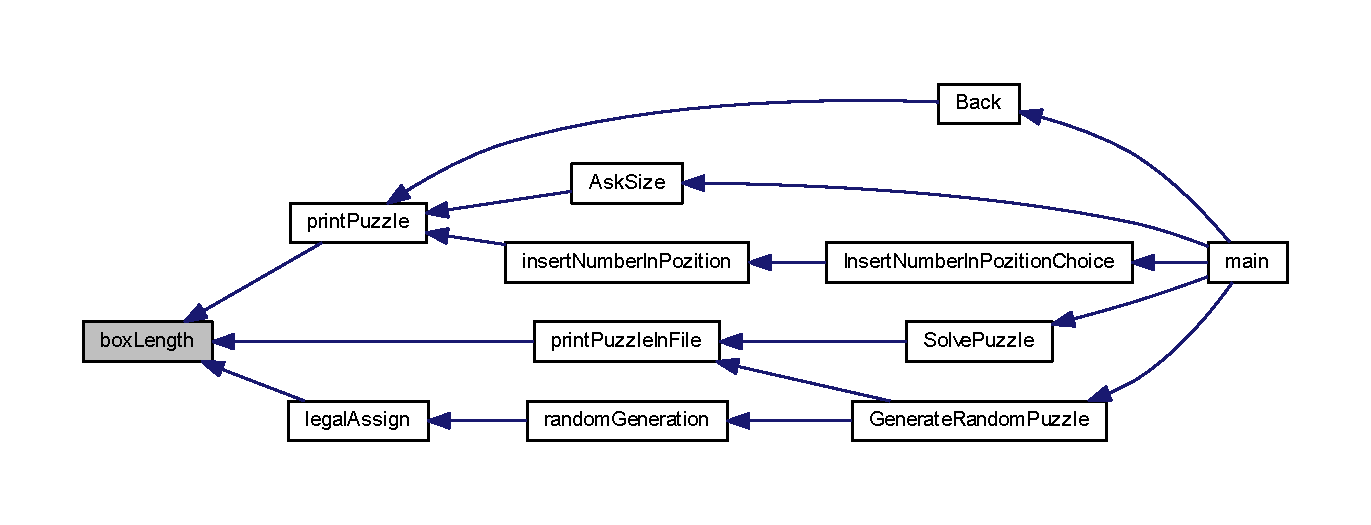
\includegraphics[width=350pt]{essential_functions_8c_a81a7d2317015b03938b3272ef99df691_icgraph}
\end{center}
\end{figure}


\index{essential\+Functions.\+c@{essential\+Functions.\+c}!copy\+Puzzle@{copy\+Puzzle}}
\index{copy\+Puzzle@{copy\+Puzzle}!essential\+Functions.\+c@{essential\+Functions.\+c}}
\subsubsection[{copy\+Puzzle(int puzzle[Size\+Of\+Puzzle][Size\+Of\+Puzzle], int copy[Size\+Of\+Puzzle][Size\+Of\+Puzzle])}]{\setlength{\rightskip}{0pt plus 5cm}void copy\+Puzzle (
\begin{DoxyParamCaption}
\item[{int}]{puzzle[\+Size\+Of\+Puzzle][\+Size\+Of\+Puzzle], }
\item[{int}]{copy[\+Size\+Of\+Puzzle][\+Size\+Of\+Puzzle]}
\end{DoxyParamCaption}
)}\label{essential_functions_8c_a8eaeede37db53451c87add11896a43c3}


A function to Back\+Up the puzzle. 


\begin{DoxyParams}{Parameters}
{\em puzzle} & The respective puzzle \\
\hline
{\em copy\+Of\+Puzzle} & \\
\hline
\end{DoxyParams}
Store the matrix into other matrix. 

Here is the caller graph for this function\+:
\nopagebreak
\begin{figure}[H]
\begin{center}
\leavevmode
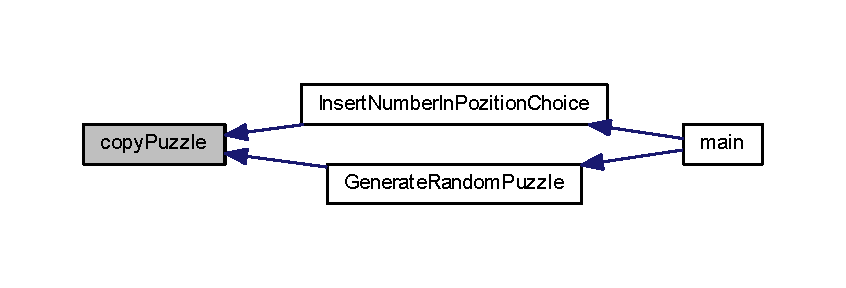
\includegraphics[width=350pt]{essential_functions_8c_a8eaeede37db53451c87add11896a43c3_icgraph}
\end{center}
\end{figure}


\index{essential\+Functions.\+c@{essential\+Functions.\+c}!counter@{counter}}
\index{counter@{counter}!essential\+Functions.\+c@{essential\+Functions.\+c}}
\subsubsection[{counter(int puzzle[Size\+Of\+Puzzle][Size\+Of\+Puzzle])}]{\setlength{\rightskip}{0pt plus 5cm}int counter (
\begin{DoxyParamCaption}
\item[{int}]{puzzle[\+Size\+Of\+Puzzle][\+Size\+Of\+Puzzle]}
\end{DoxyParamCaption}
)}\label{essential_functions_8c_aef6fed37e953a394086142cbd93bb2ad}


Counter function will return how many numbers shoud be finded in our sudoku puzzle. 


\begin{DoxyParams}{Parameters}
{\em puzzle} & The respective puzzle \\
\hline
{\em Size\+Of\+Puzzle} & Puzzle Size \\
\hline
\end{DoxyParams}
Declare a counter.

Increase counter when pozition is not equal to 0.

Return counter value. 

Here is the caller graph for this function\+:
\nopagebreak
\begin{figure}[H]
\begin{center}
\leavevmode
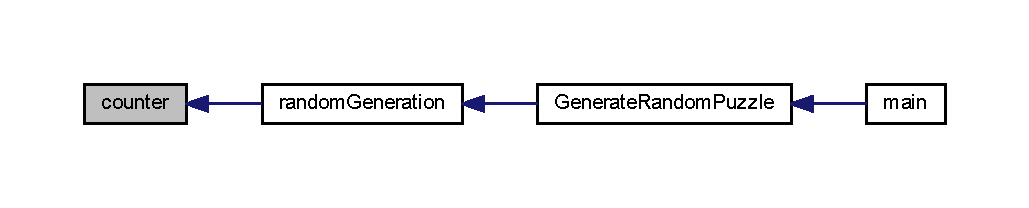
\includegraphics[width=350pt]{essential_functions_8c_aef6fed37e953a394086142cbd93bb2ad_icgraph}
\end{center}
\end{figure}


\index{essential\+Functions.\+c@{essential\+Functions.\+c}!insert\+Number\+In\+Pozition@{insert\+Number\+In\+Pozition}}
\index{insert\+Number\+In\+Pozition@{insert\+Number\+In\+Pozition}!essential\+Functions.\+c@{essential\+Functions.\+c}}
\subsubsection[{insert\+Number\+In\+Pozition(int puzzle[Size\+Of\+Puzzle][Size\+Of\+Puzzle], int Size\+Of\+Puzzle)}]{\setlength{\rightskip}{0pt plus 5cm}void insert\+Number\+In\+Pozition (
\begin{DoxyParamCaption}
\item[{int}]{puzzle[\+Size\+Of\+Puzzle][\+Size\+Of\+Puzzle], }
\item[{int}]{Size\+Of\+Puzzle}
\end{DoxyParamCaption}
)}\label{essential_functions_8c_a2b46b0b3b333036eb4dd2b48a3970f24}


Function which will insert number in specificated position. 


\begin{DoxyParams}{Parameters}
{\em puzzle} & The respective puzzle \\
\hline
{\em Size\+Of\+Puzzle} & Puzzle Size \\
\hline
\end{DoxyParams}
Use clear tool to delete the console 

Here is the call graph for this function\+:
\nopagebreak
\begin{figure}[H]
\begin{center}
\leavevmode
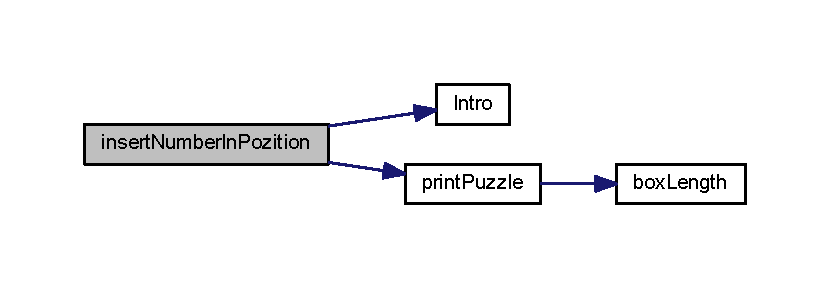
\includegraphics[width=350pt]{essential_functions_8c_a2b46b0b3b333036eb4dd2b48a3970f24_cgraph}
\end{center}
\end{figure}




Here is the caller graph for this function\+:
\nopagebreak
\begin{figure}[H]
\begin{center}
\leavevmode
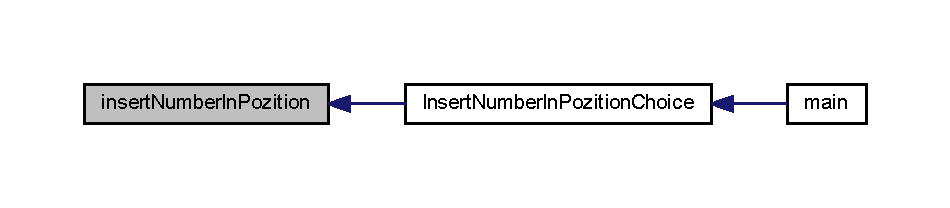
\includegraphics[width=350pt]{essential_functions_8c_a2b46b0b3b333036eb4dd2b48a3970f24_icgraph}
\end{center}
\end{figure}


\index{essential\+Functions.\+c@{essential\+Functions.\+c}!Open\+Files@{Open\+Files}}
\index{Open\+Files@{Open\+Files}!essential\+Functions.\+c@{essential\+Functions.\+c}}
\subsubsection[{Open\+Files(\+F\+I\+L\+E $\ast$file)}]{\setlength{\rightskip}{0pt plus 5cm}$\ast$ param file Data file$\ast$ bool Open\+Files (
\begin{DoxyParamCaption}
\item[{F\+I\+LE $\ast$}]{file}
\end{DoxyParamCaption}
)}\label{essential_functions_8c_afc30d97895c3f10282eb85a19c227899}


A function which will check if file is open. 

\index{essential\+Functions.\+c@{essential\+Functions.\+c}!paste\+Puzzle@{paste\+Puzzle}}
\index{paste\+Puzzle@{paste\+Puzzle}!essential\+Functions.\+c@{essential\+Functions.\+c}}
\subsubsection[{paste\+Puzzle(int puzzle[Size\+Of\+Puzzle][Size\+Of\+Puzzle], int copy[Size\+Of\+Puzzle][Size\+Of\+Puzzle])}]{\setlength{\rightskip}{0pt plus 5cm}void paste\+Puzzle (
\begin{DoxyParamCaption}
\item[{int}]{puzzle[\+Size\+Of\+Puzzle][\+Size\+Of\+Puzzle], }
\item[{int}]{copy[\+Size\+Of\+Puzzle][\+Size\+Of\+Puzzle]}
\end{DoxyParamCaption}
)}\label{essential_functions_8c_a78da4b00eb64cd00dc98f7015e13532b}


An another function to Back\+Up the puzzle. 


\begin{DoxyParams}{Parameters}
{\em puzzle} & The respective puzzle \\
\hline
{\em copy\+Of\+Puzzle} & \\
\hline
\end{DoxyParams}
Assign the backup values to puzzle. 

Here is the caller graph for this function\+:
\nopagebreak
\begin{figure}[H]
\begin{center}
\leavevmode
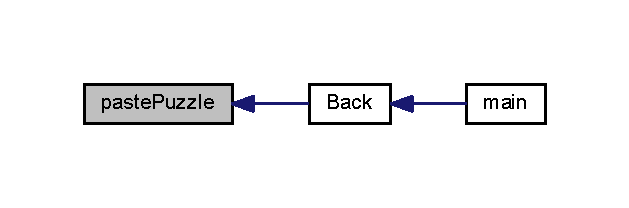
\includegraphics[width=302pt]{essential_functions_8c_a78da4b00eb64cd00dc98f7015e13532b_icgraph}
\end{center}
\end{figure}


\index{essential\+Functions.\+c@{essential\+Functions.\+c}!print\+Puzzle@{print\+Puzzle}}
\index{print\+Puzzle@{print\+Puzzle}!essential\+Functions.\+c@{essential\+Functions.\+c}}
\subsubsection[{print\+Puzzle(int puzzle[Size\+Of\+Puzzle][Size\+Of\+Puzzle], int Size\+Of\+Puzzle)}]{\setlength{\rightskip}{0pt plus 5cm}void print\+Puzzle (
\begin{DoxyParamCaption}
\item[{int}]{puzzle[\+Size\+Of\+Puzzle][\+Size\+Of\+Puzzle], }
\item[{int}]{Size\+Of\+Puzzle}
\end{DoxyParamCaption}
)}\label{essential_functions_8c_a74781138af78b469b526516a39b53959}


Function which will print puzzle. 


\begin{DoxyParams}{Parameters}
{\em puzzle} & The respective puzzle \\
\hline
{\em Size\+Of\+Puzzle} & Puzzle Size \\
\hline
\end{DoxyParams}
Get length of box.

Generate print interface. 

Here is the call graph for this function\+:
\nopagebreak
\begin{figure}[H]
\begin{center}
\leavevmode
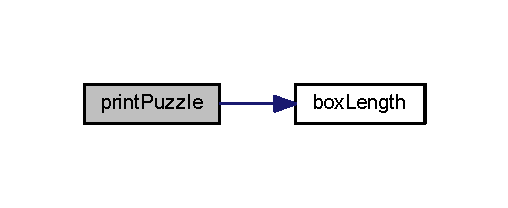
\includegraphics[width=244pt]{essential_functions_8c_a74781138af78b469b526516a39b53959_cgraph}
\end{center}
\end{figure}




Here is the caller graph for this function\+:
\nopagebreak
\begin{figure}[H]
\begin{center}
\leavevmode
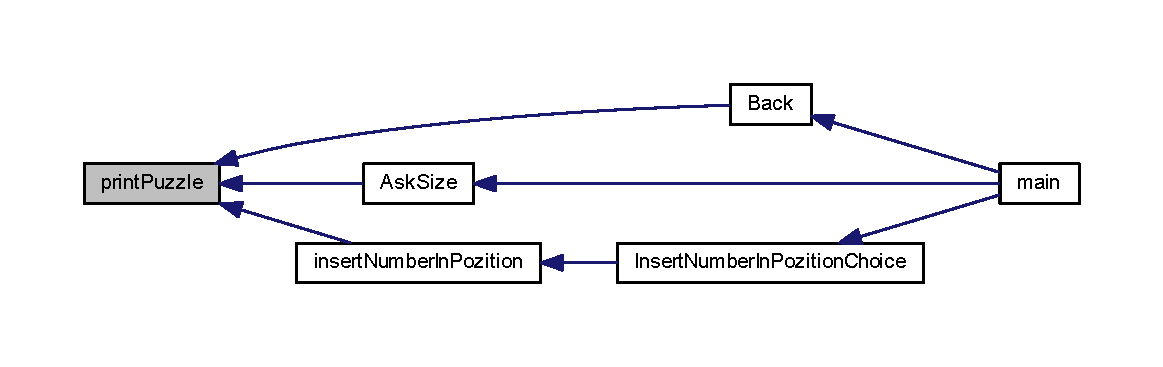
\includegraphics[width=350pt]{essential_functions_8c_a74781138af78b469b526516a39b53959_icgraph}
\end{center}
\end{figure}


\index{essential\+Functions.\+c@{essential\+Functions.\+c}!print\+Puzzle\+In\+File@{print\+Puzzle\+In\+File}}
\index{print\+Puzzle\+In\+File@{print\+Puzzle\+In\+File}!essential\+Functions.\+c@{essential\+Functions.\+c}}
\subsubsection[{print\+Puzzle\+In\+File(\+F\+I\+L\+E $\ast$filename, int puzzle[Size\+Of\+Puzzle][Size\+Of\+Puzzle], int Size\+Of\+Puzzle)}]{\setlength{\rightskip}{0pt plus 5cm}void print\+Puzzle\+In\+File (
\begin{DoxyParamCaption}
\item[{F\+I\+LE $\ast$}]{filename, }
\item[{int}]{puzzle[\+Size\+Of\+Puzzle][\+Size\+Of\+Puzzle], }
\item[{int}]{Size\+Of\+Puzzle}
\end{DoxyParamCaption}
)}\label{essential_functions_8c_a84f997248a88866cd3d6f1f6e53dc643}


Function which will print puzzle in a file. 


\begin{DoxyParams}{Parameters}
{\em filename} & Data file \\
\hline
{\em puzzle} & The respective puzzle \\
\hline
{\em Size\+Of\+Puzzle} & Puzzle Size \\
\hline
\end{DoxyParams}
Get length of box.

Generate print interface. 

Here is the call graph for this function\+:
\nopagebreak
\begin{figure}[H]
\begin{center}
\leavevmode
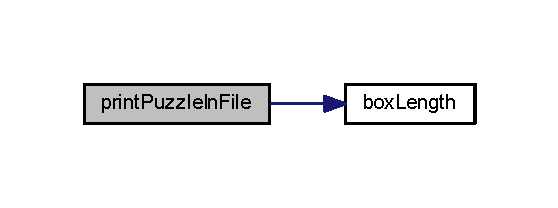
\includegraphics[width=268pt]{essential_functions_8c_a84f997248a88866cd3d6f1f6e53dc643_cgraph}
\end{center}
\end{figure}




Here is the caller graph for this function\+:
\nopagebreak
\begin{figure}[H]
\begin{center}
\leavevmode
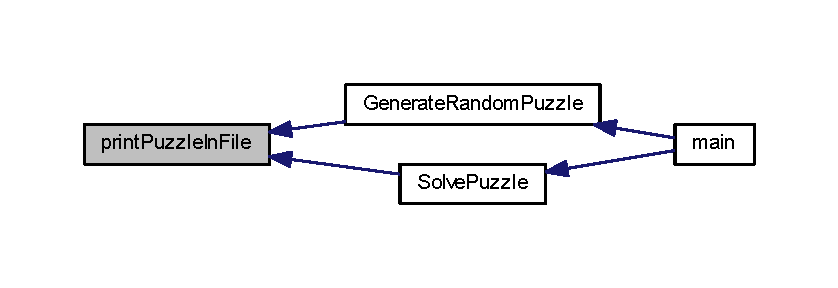
\includegraphics[width=350pt]{essential_functions_8c_a84f997248a88866cd3d6f1f6e53dc643_icgraph}
\end{center}
\end{figure}



\section{Generate\+Sudoku\+Puzzle.\+c File Reference}
\label{_generate_sudoku_puzzle_8c}\index{Generate\+Sudoku\+Puzzle.\+c@{Generate\+Sudoku\+Puzzle.\+c}}
{\ttfamily \#include \char`\"{}sudoku.\+h\char`\"{}}\\*
Include dependency graph for Generate\+Sudoku\+Puzzle.\+c\+:
\nopagebreak
\begin{figure}[H]
\begin{center}
\leavevmode
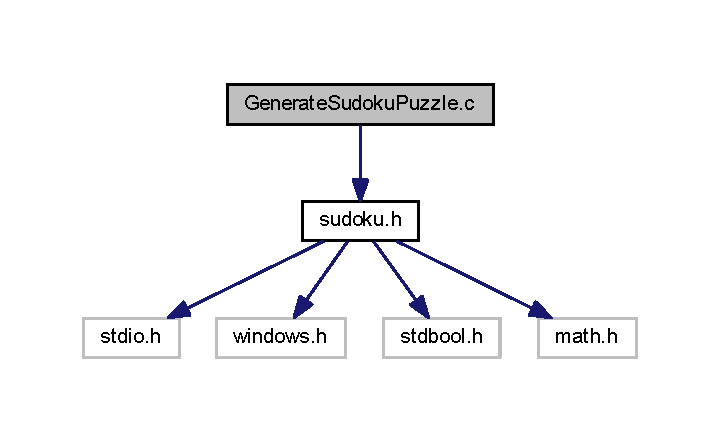
\includegraphics[width=345pt]{_generate_sudoku_puzzle_8c__incl}
\end{center}
\end{figure}
\subsection*{Functions}
\begin{DoxyCompactItemize}
\item 
bool {\bf exists\+Row} (int puzzle[{\bf Size\+Of\+Puzzle}][{\bf Size\+Of\+Puzzle}], int row, int value)
\begin{DoxyCompactList}\small\item\em There is Generation algorithm of our Sudoku puzzle, it is a simple generation using backtracking method ! \end{DoxyCompactList}\item 
bool {\bf exists\+Col} (int puzzle[{\bf Size\+Of\+Puzzle}][{\bf Size\+Of\+Puzzle}], int col, int value)
\begin{DoxyCompactList}\small\item\em Function which will check if the value exist on actual Column . \end{DoxyCompactList}\item 
bool {\bf exists\+Box} (int puzzle[{\bf Size\+Of\+Puzzle}][{\bf Size\+Of\+Puzzle}], int box\+Row, int box\+Col, int value)
\begin{DoxyCompactList}\small\item\em Function which will check if the value exist on actual box . \end{DoxyCompactList}\item 
bool {\bf legal\+Assign} (int puzzle[{\bf Size\+Of\+Puzzle}][{\bf Size\+Of\+Puzzle}], int row, int col, int value)
\begin{DoxyCompactList}\small\item\em Give permission to insert value in primary matrix. \end{DoxyCompactList}\item 
void {\bf random\+Generation} (int puzzle[{\bf Size\+Of\+Puzzle}][{\bf Size\+Of\+Puzzle}])
\begin{DoxyCompactList}\small\item\em There is Generation algorithm of our Sudoku puzzle, it is a simple generation using backtracking method ! \end{DoxyCompactList}\end{DoxyCompactItemize}


\subsection{Function Documentation}
\index{Generate\+Sudoku\+Puzzle.\+c@{Generate\+Sudoku\+Puzzle.\+c}!exists\+Box@{exists\+Box}}
\index{exists\+Box@{exists\+Box}!Generate\+Sudoku\+Puzzle.\+c@{Generate\+Sudoku\+Puzzle.\+c}}
\subsubsection[{exists\+Box(int puzzle[Size\+Of\+Puzzle][Size\+Of\+Puzzle], int box\+Row, int box\+Col, int value)}]{\setlength{\rightskip}{0pt plus 5cm}bool exists\+Box (
\begin{DoxyParamCaption}
\item[{int}]{puzzle[\+Size\+Of\+Puzzle][\+Size\+Of\+Puzzle], }
\item[{int}]{box\+Row, }
\item[{int}]{box\+Col, }
\item[{int}]{value}
\end{DoxyParamCaption}
)}\label{_generate_sudoku_puzzle_8c_abf81a768e692f635d7c0dd855240921a}


Function which will check if the value exist on actual box . 


\begin{DoxyParams}{Parameters}
{\em puzzle} & The respective puzzle \\
\hline
{\em Box\+Row} & \\
\hline
{\em Box\+Col} & \\
\hline
{\em Value} & The value of number \\
\hline
\end{DoxyParams}


Here is the caller graph for this function\+:
\nopagebreak
\begin{figure}[H]
\begin{center}
\leavevmode
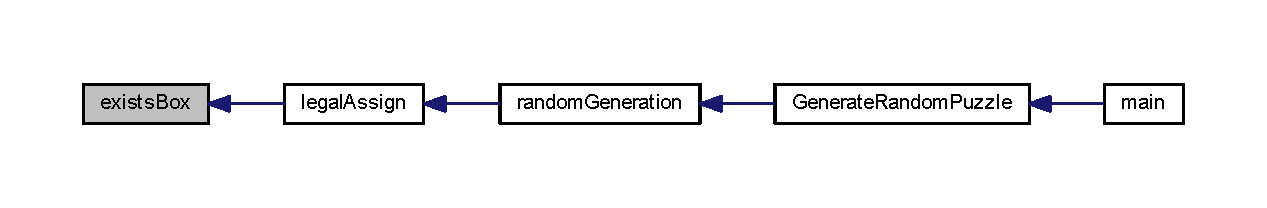
\includegraphics[width=350pt]{_generate_sudoku_puzzle_8c_abf81a768e692f635d7c0dd855240921a_icgraph}
\end{center}
\end{figure}


\index{Generate\+Sudoku\+Puzzle.\+c@{Generate\+Sudoku\+Puzzle.\+c}!exists\+Col@{exists\+Col}}
\index{exists\+Col@{exists\+Col}!Generate\+Sudoku\+Puzzle.\+c@{Generate\+Sudoku\+Puzzle.\+c}}
\subsubsection[{exists\+Col(int puzzle[Size\+Of\+Puzzle][Size\+Of\+Puzzle], int col, int value)}]{\setlength{\rightskip}{0pt plus 5cm}bool exists\+Col (
\begin{DoxyParamCaption}
\item[{int}]{puzzle[\+Size\+Of\+Puzzle][\+Size\+Of\+Puzzle], }
\item[{int}]{col, }
\item[{int}]{value}
\end{DoxyParamCaption}
)}\label{_generate_sudoku_puzzle_8c_aed140ba5f01d4c8cf24ad69b22a700d8}


Function which will check if the value exist on actual Column . 


\begin{DoxyParams}{Parameters}
{\em puzzle} & The respective puzzle \\
\hline
{\em Column} & Respective Column \\
\hline
{\em Value} & The value of number \\
\hline
\end{DoxyParams}


Here is the caller graph for this function\+:
\nopagebreak
\begin{figure}[H]
\begin{center}
\leavevmode
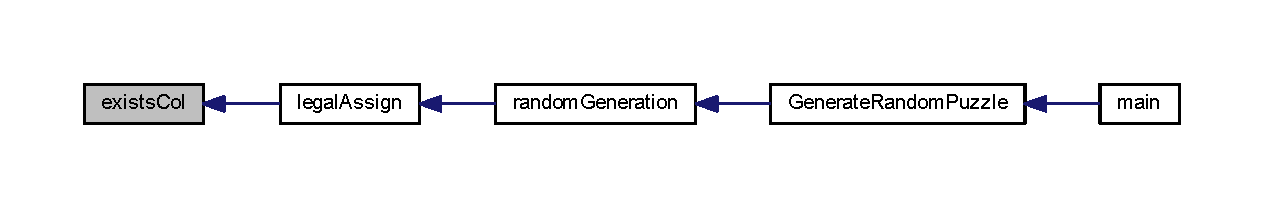
\includegraphics[width=350pt]{_generate_sudoku_puzzle_8c_aed140ba5f01d4c8cf24ad69b22a700d8_icgraph}
\end{center}
\end{figure}


\index{Generate\+Sudoku\+Puzzle.\+c@{Generate\+Sudoku\+Puzzle.\+c}!exists\+Row@{exists\+Row}}
\index{exists\+Row@{exists\+Row}!Generate\+Sudoku\+Puzzle.\+c@{Generate\+Sudoku\+Puzzle.\+c}}
\subsubsection[{exists\+Row(int puzzle[Size\+Of\+Puzzle][Size\+Of\+Puzzle], int row, int value)}]{\setlength{\rightskip}{0pt plus 5cm}bool exists\+Row (
\begin{DoxyParamCaption}
\item[{int}]{puzzle[\+Size\+Of\+Puzzle][\+Size\+Of\+Puzzle], }
\item[{int}]{row, }
\item[{int}]{value}
\end{DoxyParamCaption}
)}\label{_generate_sudoku_puzzle_8c_a3d79c9c1f77209505ee449e8c6bc5ab2}


There is Generation algorithm of our Sudoku puzzle, it is a simple generation using backtracking method ! 

Function which will check if the value exist on actual Row . 
\begin{DoxyParams}{Parameters}
{\em puzzle} & The respective puzzle \\
\hline
{\em Row} & Respective Row \\
\hline
{\em Value} & The value of number \\
\hline
\end{DoxyParams}


Here is the caller graph for this function\+:
\nopagebreak
\begin{figure}[H]
\begin{center}
\leavevmode
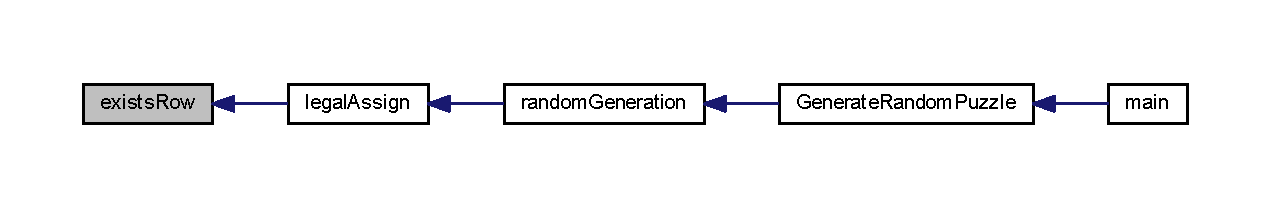
\includegraphics[width=350pt]{_generate_sudoku_puzzle_8c_a3d79c9c1f77209505ee449e8c6bc5ab2_icgraph}
\end{center}
\end{figure}


\index{Generate\+Sudoku\+Puzzle.\+c@{Generate\+Sudoku\+Puzzle.\+c}!legal\+Assign@{legal\+Assign}}
\index{legal\+Assign@{legal\+Assign}!Generate\+Sudoku\+Puzzle.\+c@{Generate\+Sudoku\+Puzzle.\+c}}
\subsubsection[{legal\+Assign(int puzzle[Size\+Of\+Puzzle][Size\+Of\+Puzzle], int row, int col, int value)}]{\setlength{\rightskip}{0pt plus 5cm}bool legal\+Assign (
\begin{DoxyParamCaption}
\item[{int}]{puzzle[\+Size\+Of\+Puzzle][\+Size\+Of\+Puzzle], }
\item[{int}]{row, }
\item[{int}]{col, }
\item[{int}]{value}
\end{DoxyParamCaption}
)}\label{_generate_sudoku_puzzle_8c_a267a6d32821d62a5184da4855cb03091}


Give permission to insert value in primary matrix. 


\begin{DoxyParams}{Parameters}
{\em puzzle} & The respective puzzle \\
\hline
{\em Row} & Respective Row \\
\hline
{\em Value} & The value of number \\
\hline
{\em Value} & The value of number \\
\hline
\end{DoxyParams}
Get size of box 

Here is the call graph for this function\+:
\nopagebreak
\begin{figure}[H]
\begin{center}
\leavevmode
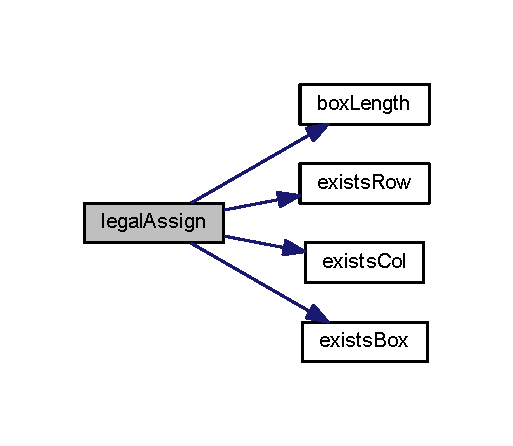
\includegraphics[width=246pt]{_generate_sudoku_puzzle_8c_a267a6d32821d62a5184da4855cb03091_cgraph}
\end{center}
\end{figure}




Here is the caller graph for this function\+:
\nopagebreak
\begin{figure}[H]
\begin{center}
\leavevmode
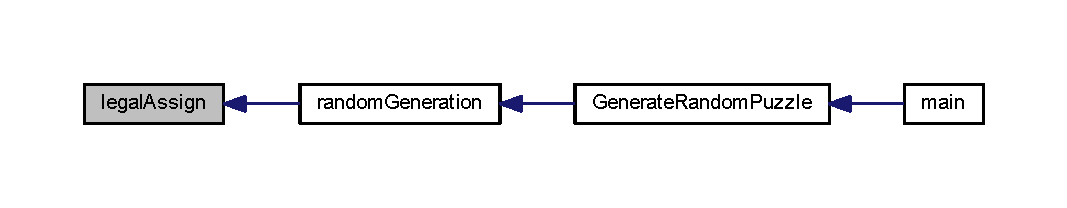
\includegraphics[width=350pt]{_generate_sudoku_puzzle_8c_a267a6d32821d62a5184da4855cb03091_icgraph}
\end{center}
\end{figure}


\index{Generate\+Sudoku\+Puzzle.\+c@{Generate\+Sudoku\+Puzzle.\+c}!random\+Generation@{random\+Generation}}
\index{random\+Generation@{random\+Generation}!Generate\+Sudoku\+Puzzle.\+c@{Generate\+Sudoku\+Puzzle.\+c}}
\subsubsection[{random\+Generation(int puzzle[Size\+Of\+Puzzle][Size\+Of\+Puzzle])}]{\setlength{\rightskip}{0pt plus 5cm}void random\+Generation (
\begin{DoxyParamCaption}
\item[{int}]{puzzle[\+Size\+Of\+Puzzle][\+Size\+Of\+Puzzle]}
\end{DoxyParamCaption}
)}\label{_generate_sudoku_puzzle_8c_a6a49f0a7a0398f2659d6642120ea48dc}


There is Generation algorithm of our Sudoku puzzle, it is a simple generation using backtracking method ! 


\begin{DoxyParams}{Parameters}
{\em puzzle} & The respective puzzle \\
\hline
\end{DoxyParams}
Random seed by clock.

Generate random numbers on rows !

Generate random numbers on columns !

Generate a value which will fill matrix !

Get rights to assign value

Assign the value

Declare a variable which will store how much numbers are avaiable on matrix. 

Here is the call graph for this function\+:
\nopagebreak
\begin{figure}[H]
\begin{center}
\leavevmode
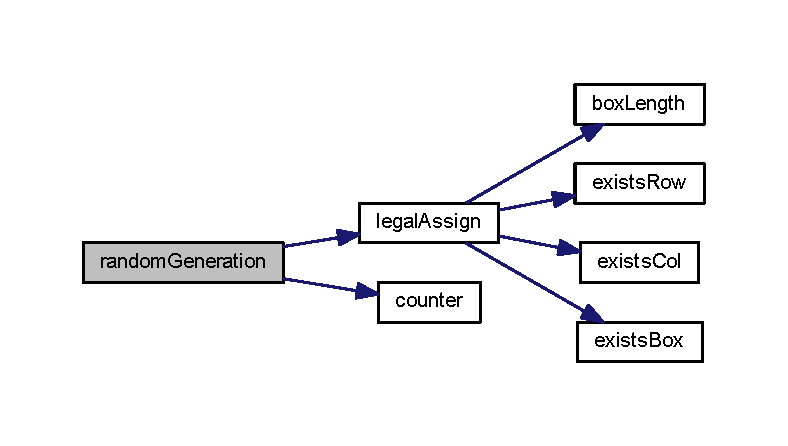
\includegraphics[width=350pt]{_generate_sudoku_puzzle_8c_a6a49f0a7a0398f2659d6642120ea48dc_cgraph}
\end{center}
\end{figure}




Here is the caller graph for this function\+:
\nopagebreak
\begin{figure}[H]
\begin{center}
\leavevmode
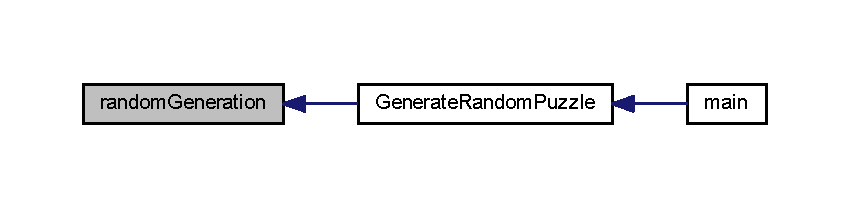
\includegraphics[width=350pt]{_generate_sudoku_puzzle_8c_a6a49f0a7a0398f2659d6642120ea48dc_icgraph}
\end{center}
\end{figure}



\section{main.\+c File Reference}
\label{main_8c}\index{main.\+c@{main.\+c}}
{\ttfamily \#include \char`\"{}sudoku.\+h\char`\"{}}\\*
Include dependency graph for main.\+c\+:
\nopagebreak
\begin{figure}[H]
\begin{center}
\leavevmode
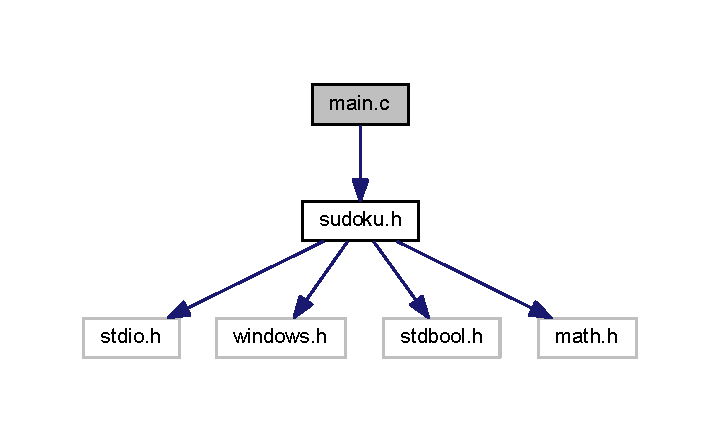
\includegraphics[width=345pt]{main_8c__incl}
\end{center}
\end{figure}
\subsection*{Functions}
\begin{DoxyCompactItemize}
\item 
int {\bf main} ()
\end{DoxyCompactItemize}


\subsection{Function Documentation}
\index{main.\+c@{main.\+c}!main@{main}}
\index{main@{main}!main.\+c@{main.\+c}}
\subsubsection[{main()}]{\setlength{\rightskip}{0pt plus 5cm}int main (
\begin{DoxyParamCaption}
{}
\end{DoxyParamCaption}
)}\label{main_8c_ae66f6b31b5ad750f1fe042a706a4e3d4}
Create Interface of Program

Here is generated the puzzle full with 0 

Here is the call graph for this function\+:
\nopagebreak
\begin{figure}[H]
\begin{center}
\leavevmode
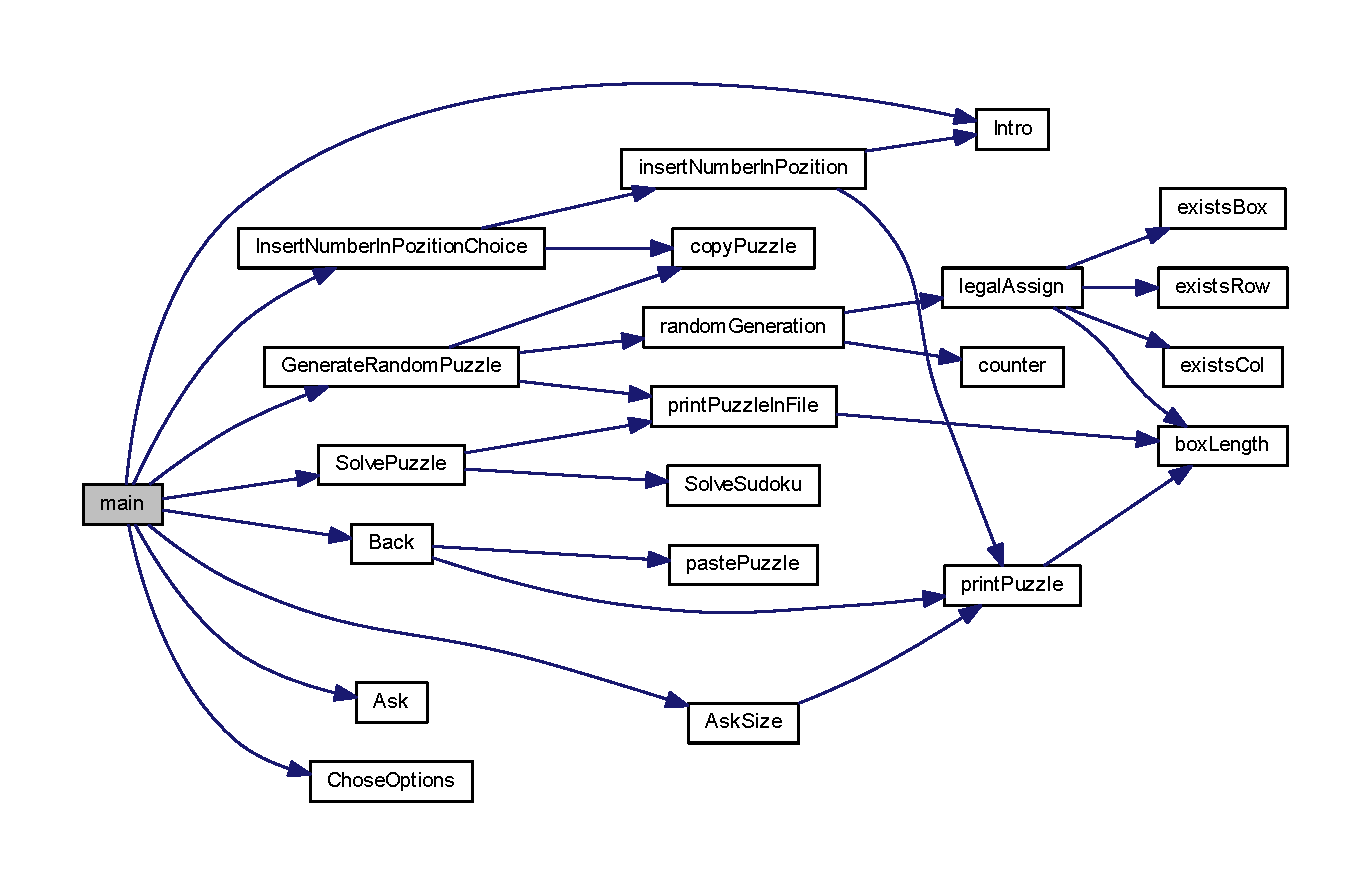
\includegraphics[width=350pt]{main_8c_ae66f6b31b5ad750f1fe042a706a4e3d4_cgraph}
\end{center}
\end{figure}



\section{sudoku.\+h File Reference}
\label{sudoku_8h}\index{sudoku.\+h@{sudoku.\+h}}
{\ttfamily \#include $<$stdio.\+h$>$}\\*
{\ttfamily \#include $<$windows.\+h$>$}\\*
{\ttfamily \#include $<$stdbool.\+h$>$}\\*
{\ttfamily \#include $<$math.\+h$>$}\\*
Include dependency graph for sudoku.\+h\+:
\nopagebreak
\begin{figure}[H]
\begin{center}
\leavevmode
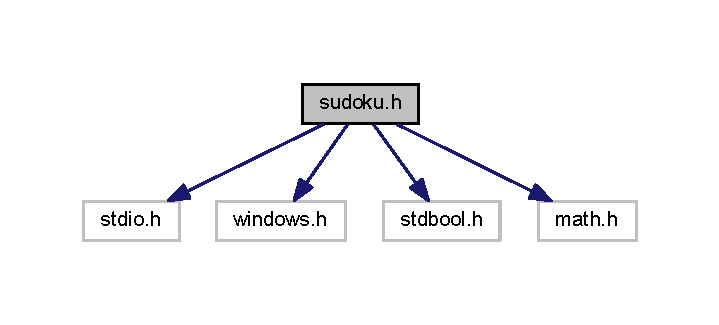
\includegraphics[width=345pt]{sudoku_8h__incl}
\end{center}
\end{figure}
This graph shows which files directly or indirectly include this file\+:
\nopagebreak
\begin{figure}[H]
\begin{center}
\leavevmode
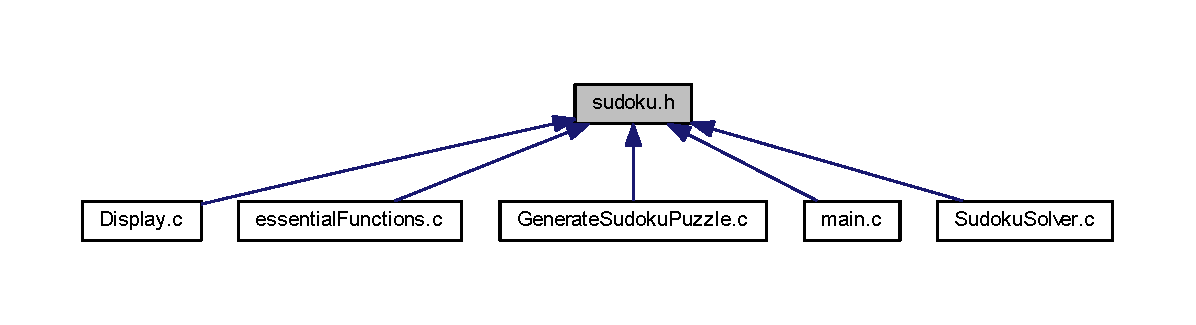
\includegraphics[width=350pt]{sudoku_8h__dep__incl}
\end{center}
\end{figure}
\subsection*{Macros}
\begin{DoxyCompactItemize}
\item 
\#define {\bf U\+N\+A\+S\+S\+I\+G\+N\+ED}~0
\end{DoxyCompactItemize}
\subsection*{Variables}
\begin{DoxyCompactItemize}
\item 
int {\bf Size\+Of\+Puzzle}
\item 
bool {\bf Game\+Over}
\item 
bool {\bf Start}
\item 
int {\bf choice}
\item 
int {\bf number\+Of\+Solutions}
\item 
int {\bf solution}
\item 
int {\bf iterations}
\end{DoxyCompactItemize}


\subsection{Macro Definition Documentation}
\index{sudoku.\+h@{sudoku.\+h}!U\+N\+A\+S\+S\+I\+G\+N\+ED@{U\+N\+A\+S\+S\+I\+G\+N\+ED}}
\index{U\+N\+A\+S\+S\+I\+G\+N\+ED@{U\+N\+A\+S\+S\+I\+G\+N\+ED}!sudoku.\+h@{sudoku.\+h}}
\subsubsection[{U\+N\+A\+S\+S\+I\+G\+N\+ED}]{\setlength{\rightskip}{0pt plus 5cm}\#define U\+N\+A\+S\+S\+I\+G\+N\+ED~0}\label{sudoku_8h_a7f2a734b84f750bb35708fd8f3d0121e}


\subsection{Variable Documentation}
\index{sudoku.\+h@{sudoku.\+h}!choice@{choice}}
\index{choice@{choice}!sudoku.\+h@{sudoku.\+h}}
\subsubsection[{choice}]{\setlength{\rightskip}{0pt plus 5cm}int choice}\label{sudoku_8h_a63bd75f20c553f0d65d7bb29b3f35696}
Interface status \index{sudoku.\+h@{sudoku.\+h}!Game\+Over@{Game\+Over}}
\index{Game\+Over@{Game\+Over}!sudoku.\+h@{sudoku.\+h}}
\subsubsection[{Game\+Over}]{\setlength{\rightskip}{0pt plus 5cm}bool Game\+Over}\label{sudoku_8h_a24624e67404a49abae1a7cc8b96f7add}
Size of puzzle \index{sudoku.\+h@{sudoku.\+h}!iterations@{iterations}}
\index{iterations@{iterations}!sudoku.\+h@{sudoku.\+h}}
\subsubsection[{iterations}]{\setlength{\rightskip}{0pt plus 5cm}int iterations}\label{sudoku_8h_a1d10e252e778731e59f0f71afd7e727e}
\index{sudoku.\+h@{sudoku.\+h}!number\+Of\+Solutions@{number\+Of\+Solutions}}
\index{number\+Of\+Solutions@{number\+Of\+Solutions}!sudoku.\+h@{sudoku.\+h}}
\subsubsection[{number\+Of\+Solutions}]{\setlength{\rightskip}{0pt plus 5cm}int number\+Of\+Solutions}\label{sudoku_8h_a03012dc31899ca10a8626db3a3820ad8}
Choice status for switch statements \index{sudoku.\+h@{sudoku.\+h}!Size\+Of\+Puzzle@{Size\+Of\+Puzzle}}
\index{Size\+Of\+Puzzle@{Size\+Of\+Puzzle}!sudoku.\+h@{sudoku.\+h}}
\subsubsection[{Size\+Of\+Puzzle}]{\setlength{\rightskip}{0pt plus 5cm}int Size\+Of\+Puzzle}\label{sudoku_8h_ab651976d7f8811d64f361a3494db3c15}
\index{sudoku.\+h@{sudoku.\+h}!solution@{solution}}
\index{solution@{solution}!sudoku.\+h@{sudoku.\+h}}
\subsubsection[{solution}]{\setlength{\rightskip}{0pt plus 5cm}int solution}\label{sudoku_8h_a31c1b12669214beebfa1ee8ef0ba9347}
\index{sudoku.\+h@{sudoku.\+h}!Start@{Start}}
\index{Start@{Start}!sudoku.\+h@{sudoku.\+h}}
\subsubsection[{Start}]{\setlength{\rightskip}{0pt plus 5cm}bool Start}\label{sudoku_8h_ab26d55e5cf0450b0147af1eea20a0723}
Game status 
\section{Sudoku\+Solver.\+c File Reference}
\label{_sudoku_solver_8c}\index{Sudoku\+Solver.\+c@{Sudoku\+Solver.\+c}}
{\ttfamily \#include \char`\"{}sudoku.\+h\char`\"{}}\\*
Include dependency graph for Sudoku\+Solver.\+c\+:
\nopagebreak
\begin{figure}[H]
\begin{center}
\leavevmode
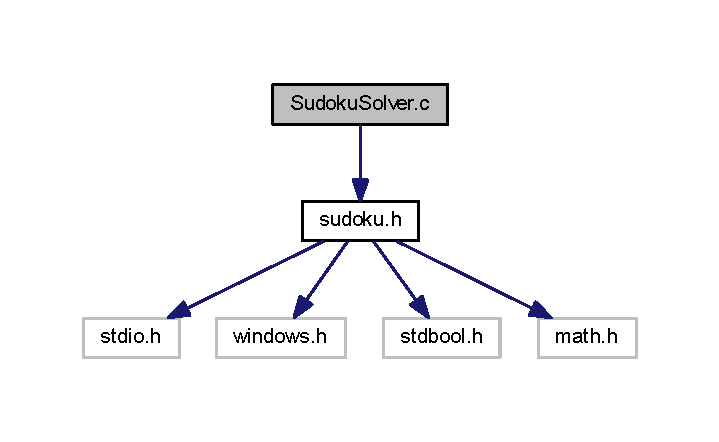
\includegraphics[width=345pt]{_sudoku_solver_8c__incl}
\end{center}
\end{figure}
\subsection*{Functions}
\begin{DoxyCompactItemize}
\item 
int {\bf Find\+Unassigned} (int puzzle[{\bf Size\+Of\+Puzzle}][{\bf Size\+Of\+Puzzle}], int $\ast$row, int $\ast$col)
\begin{DoxyCompactList}\small\item\em Starting counter of solution. \end{DoxyCompactList}\item 
int {\bf is\+Safe} (int puzzle[{\bf Size\+Of\+Puzzle}][{\bf Size\+Of\+Puzzle}], int row, int col, int num)
\begin{DoxyCompactList}\small\item\em Returns a boolean which indicates whether it will be legal to assign num to the given row,col location. \end{DoxyCompactList}\item 
int {\bf Used\+In\+Row} (int puzzle[{\bf Size\+Of\+Puzzle}][{\bf Size\+Of\+Puzzle}], int row, int num)
\begin{DoxyCompactList}\small\item\em Returns a boolean which indicates whether any assigned entry in the specified row matches the given number. \end{DoxyCompactList}\item 
int {\bf Used\+In\+Col} (int puzzle[{\bf Size\+Of\+Puzzle}][{\bf Size\+Of\+Puzzle}], int col, int num)
\begin{DoxyCompactList}\small\item\em Returns a boolean which indicates whether any assigned entry in the specified column matches the given number. \end{DoxyCompactList}\item 
int {\bf Used\+In\+Box} (int puzzle[{\bf Size\+Of\+Puzzle}][{\bf Size\+Of\+Puzzle}], int Box\+Start\+Row, int Box\+Start\+Col, int num)
\begin{DoxyCompactList}\small\item\em Returns a boolean which indicates whether any assigned entry within the specified box matches the given number. \end{DoxyCompactList}\item 
int {\bf Solve\+Sudoku} (int puzzle[{\bf Size\+Of\+Puzzle}][{\bf Size\+Of\+Puzzle}], F\+I\+LE $\ast$file\+Name)
\begin{DoxyCompactList}\small\item\em Takes a partially filled-\/in grid and attempts to assign values to all unassigned locations in such a way to meet the requirements for Sudoku solution (non-\/duplication across rows, columns, and boxes) \end{DoxyCompactList}\end{DoxyCompactItemize}
\subsection*{Variables}
\begin{DoxyCompactItemize}
\item 
{\bf solution} = 0
\end{DoxyCompactItemize}


\subsection{Function Documentation}
\index{Sudoku\+Solver.\+c@{Sudoku\+Solver.\+c}!Find\+Unassigned@{Find\+Unassigned}}
\index{Find\+Unassigned@{Find\+Unassigned}!Sudoku\+Solver.\+c@{Sudoku\+Solver.\+c}}
\subsubsection[{Find\+Unassigned(int puzzle[Size\+Of\+Puzzle][Size\+Of\+Puzzle], int $\ast$row, int $\ast$col)}]{\setlength{\rightskip}{0pt plus 5cm}int Find\+Unassigned (
\begin{DoxyParamCaption}
\item[{int}]{puzzle[\+Size\+Of\+Puzzle][\+Size\+Of\+Puzzle], }
\item[{int $\ast$}]{row, }
\item[{int $\ast$}]{col}
\end{DoxyParamCaption}
)}\label{_sudoku_solver_8c_a264ad167884b95d76b9e9435cc12ea27}


Starting counter of solution. 

Searches the puzzle to find an entry that is still unassigned. If found, the reference parameters row, col will be set the location that is unassigned, and true is returned. If no unassigned entries remain, false is returned. 
\begin{DoxyParams}{Parameters}
{\em puzzle} & The respective puzzle \\
\hline
{\em Row} & \\
\hline
{\em Column} & \\
\hline
\end{DoxyParams}
\index{Sudoku\+Solver.\+c@{Sudoku\+Solver.\+c}!is\+Safe@{is\+Safe}}
\index{is\+Safe@{is\+Safe}!Sudoku\+Solver.\+c@{Sudoku\+Solver.\+c}}
\subsubsection[{is\+Safe(int puzzle[Size\+Of\+Puzzle][Size\+Of\+Puzzle], int row, int col, int num)}]{\setlength{\rightskip}{0pt plus 5cm}int is\+Safe (
\begin{DoxyParamCaption}
\item[{int}]{puzzle[\+Size\+Of\+Puzzle][\+Size\+Of\+Puzzle], }
\item[{int}]{row, }
\item[{int}]{col, }
\item[{int}]{num}
\end{DoxyParamCaption}
)}\label{_sudoku_solver_8c_abb05c837f81a61dbbfeac9d51084f1d2}


Returns a boolean which indicates whether it will be legal to assign num to the given row,col location. 


\begin{DoxyParams}{Parameters}
{\em puzzle} & The respective puzzle \\
\hline
{\em Row} & \\
\hline
{\em Column} & \\
\hline
{\em Number} & \\
\hline
\end{DoxyParams}
Check if \textquotesingle{}num\textquotesingle{} is not already placed in current row, current column and current box \index{Sudoku\+Solver.\+c@{Sudoku\+Solver.\+c}!Solve\+Sudoku@{Solve\+Sudoku}}
\index{Solve\+Sudoku@{Solve\+Sudoku}!Sudoku\+Solver.\+c@{Sudoku\+Solver.\+c}}
\subsubsection[{Solve\+Sudoku(int puzzle[Size\+Of\+Puzzle][Size\+Of\+Puzzle], F\+I\+L\+E $\ast$file\+Name)}]{\setlength{\rightskip}{0pt plus 5cm}int Solve\+Sudoku (
\begin{DoxyParamCaption}
\item[{int}]{puzzle[\+Size\+Of\+Puzzle][\+Size\+Of\+Puzzle], }
\item[{F\+I\+LE $\ast$}]{file\+Name}
\end{DoxyParamCaption}
)}\label{_sudoku_solver_8c_a293f5b647b84feea43bb245b3b56987e}


Takes a partially filled-\/in grid and attempts to assign values to all unassigned locations in such a way to meet the requirements for Sudoku solution (non-\/duplication across rows, columns, and boxes) 


\begin{DoxyParams}{Parameters}
{\em puzzle} & The respective puzzle \\
\hline
{\em file} & Data file \\
\hline
\end{DoxyParams}
If there is no unassigned location, we are done

Starting counter of iteraions

Consider digits 1 to Size\+Of\+Puzzle

If looks promising

Make tentative assignment

Return, if success

Failure, unmake \& try again

This triggers backtracking 

Here is the caller graph for this function\+:
\nopagebreak
\begin{figure}[H]
\begin{center}
\leavevmode
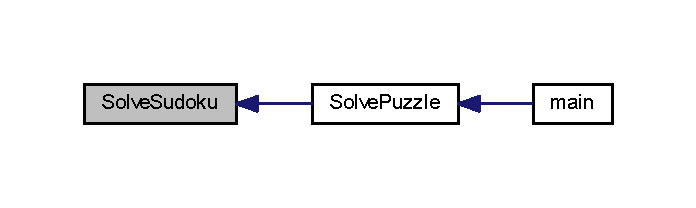
\includegraphics[width=334pt]{_sudoku_solver_8c_a293f5b647b84feea43bb245b3b56987e_icgraph}
\end{center}
\end{figure}


\index{Sudoku\+Solver.\+c@{Sudoku\+Solver.\+c}!Used\+In\+Box@{Used\+In\+Box}}
\index{Used\+In\+Box@{Used\+In\+Box}!Sudoku\+Solver.\+c@{Sudoku\+Solver.\+c}}
\subsubsection[{Used\+In\+Box(int puzzle[Size\+Of\+Puzzle][Size\+Of\+Puzzle], int Box\+Start\+Row, int Box\+Start\+Col, int num)}]{\setlength{\rightskip}{0pt plus 5cm}int Used\+In\+Box (
\begin{DoxyParamCaption}
\item[{int}]{puzzle[\+Size\+Of\+Puzzle][\+Size\+Of\+Puzzle], }
\item[{int}]{Box\+Start\+Row, }
\item[{int}]{Box\+Start\+Col, }
\item[{int}]{num}
\end{DoxyParamCaption}
)}\label{_sudoku_solver_8c_a91648104e1cecc5abbf65d060233ff14}


Returns a boolean which indicates whether any assigned entry within the specified box matches the given number. 


\begin{DoxyParams}{Parameters}
{\em puzzle} & The respective puzzle \\
\hline
{\em Box\+Start\+Row} & \\
\hline
{\em Box\+Start\+Col} & \\
\hline
{\em Number} & \\
\hline
\end{DoxyParams}
\index{Sudoku\+Solver.\+c@{Sudoku\+Solver.\+c}!Used\+In\+Col@{Used\+In\+Col}}
\index{Used\+In\+Col@{Used\+In\+Col}!Sudoku\+Solver.\+c@{Sudoku\+Solver.\+c}}
\subsubsection[{Used\+In\+Col(int puzzle[Size\+Of\+Puzzle][Size\+Of\+Puzzle], int col, int num)}]{\setlength{\rightskip}{0pt plus 5cm}int Used\+In\+Col (
\begin{DoxyParamCaption}
\item[{int}]{puzzle[\+Size\+Of\+Puzzle][\+Size\+Of\+Puzzle], }
\item[{int}]{col, }
\item[{int}]{num}
\end{DoxyParamCaption}
)}\label{_sudoku_solver_8c_a25ad8cfbe4bddf48da5ab746075f7d82}


Returns a boolean which indicates whether any assigned entry in the specified column matches the given number. 


\begin{DoxyParams}{Parameters}
{\em puzzle} & The respective puzzle \\
\hline
{\em Column} & \\
\hline
{\em Number} & \\
\hline
\end{DoxyParams}
\index{Sudoku\+Solver.\+c@{Sudoku\+Solver.\+c}!Used\+In\+Row@{Used\+In\+Row}}
\index{Used\+In\+Row@{Used\+In\+Row}!Sudoku\+Solver.\+c@{Sudoku\+Solver.\+c}}
\subsubsection[{Used\+In\+Row(int puzzle[Size\+Of\+Puzzle][Size\+Of\+Puzzle], int row, int num)}]{\setlength{\rightskip}{0pt plus 5cm}int Used\+In\+Row (
\begin{DoxyParamCaption}
\item[{int}]{puzzle[\+Size\+Of\+Puzzle][\+Size\+Of\+Puzzle], }
\item[{int}]{row, }
\item[{int}]{num}
\end{DoxyParamCaption}
)}\label{_sudoku_solver_8c_a4d142a58dac91af1a49be769d96ac456}


Returns a boolean which indicates whether any assigned entry in the specified row matches the given number. 


\begin{DoxyParams}{Parameters}
{\em puzzle} & The respective puzzle \\
\hline
{\em Row} & \\
\hline
{\em Number} & \\
\hline
\end{DoxyParams}


\subsection{Variable Documentation}
\index{Sudoku\+Solver.\+c@{Sudoku\+Solver.\+c}!solution@{solution}}
\index{solution@{solution}!Sudoku\+Solver.\+c@{Sudoku\+Solver.\+c}}
\subsubsection[{solution}]{\setlength{\rightskip}{0pt plus 5cm}solution = 0}\label{_sudoku_solver_8c_ae4bd085d10e18fd066c9ff3e6af72173}

%--- End generated contents ---

% Index
\backmatter
\newpage
\phantomsection
\clearemptydoublepage
\addcontentsline{toc}{chapter}{Index}
\printindex

\end{document}
